% Compile with latex, then dvisvgm --no-fonts --exact --bbox=papersize.
\documentclass[tikz,border=8pt]{standalone}
\usepackage[T1]{fontenc}
\usepackage{lmodern}
\usetikzlibrary{arrows.meta}
\begin{document}
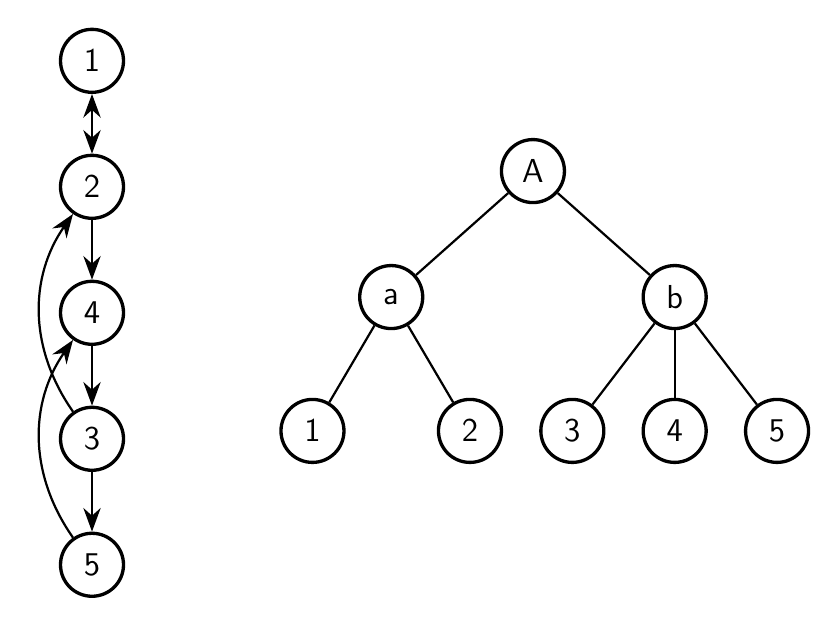
\begin{tikzpicture}[
    font=\sffamily\large,
    vertex/.style={circle,draw,line width=1.2pt,fill=white,
                   minimum size=8mm,inner sep=0pt},
    edge/.style={line width=0.8pt},
    directed/.style={edge,-{Stealth[length=3mm,width=2.2mm]}}]
  % Original strongly connected graph: cycles (1,2) and (4,3,5).
  \node[vertex] (1) at (0,0) {1};
  \node[vertex] (2) at (0,-1.6) {2};
  \node[vertex] (4) at (0,-3.2) {4};
  \node[vertex] (3) at (0,-4.8) {3};
  \node[vertex] (5) at (0,-6.4) {5};
  \draw[edge,{Stealth[length=3mm,width=2.2mm]}-{Stealth[length=3mm,width=2.2mm]}] (1) -- (2);
  \draw[directed] (2) -- (4);
  \draw[directed] (4) -- (3);
  \draw[directed] (3) -- (5);
  \draw[directed] (3) to[bend left=35] (2);
  \draw[directed] (5) to[bend left=35] (4);
  % Contraction tree: a={1,2}, b={3,4,5}, A={a,b}.
  \node[vertex] (A) at (5.6,-1.4) {A};
  \node[vertex] (a) at (3.8,-3) {a};
  \node[vertex] (b) at (7.4,-3) {b};
  \node[vertex] (leaf1) at (2.8,-4.7) {1};
  \node[vertex] (leaf2) at (4.8,-4.7) {2};
  \node[vertex] (leaf3) at (6.1,-4.7) {3};
  \node[vertex] (leaf4) at (7.4,-4.7) {4};
  \node[vertex] (leaf5) at (8.7,-4.7) {5};
  \draw[edge] (A) -- (a) -- (leaf1);
  \draw[edge] (a) -- (leaf2);
  \draw[edge] (A) -- (b) -- (leaf3);
  \draw[edge] (b) -- (leaf4);
  \draw[edge] (b) -- (leaf5);
\end{tikzpicture}
\end{document}
